\tikzstyle{inputNode}=[draw,circle,minimum size=17pt,inner sep=0pt]
\tikzstyle{stateTransition}=[-stealth, thick]

%\begin{document}
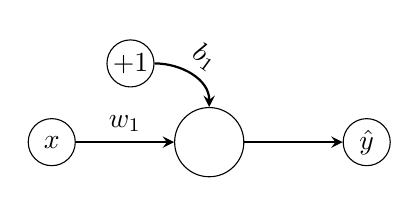
\begin{tikzpicture}
	\node[draw,circle,minimum size=25pt,inner sep=0pt] (x) at (0,0) {};

	\node[inputNode] (x0) at (-1, 1) {$\tiny +1$};
	\node[inputNode] (x1) at (-2, 0) {$\tiny x$};
	\node[inputNode] (y) at (2, 0) {$\tiny \hat{y}$};
	
	\draw[stateTransition] (x0) to[out=0,in=90] node [midway, sloped, above] {$b_{1}$} (x);
	\draw[stateTransition] (x1) to[out=0,in=180] node [midway, sloped, above] {$w_{1}$} (x);
	\draw[stateTransition] (x) to[out=0,in=180] node [midway, sloped, above] {} (y);

	
\end{tikzpicture}